% \documentclass[10pt,twocolumn]{article}
\documentclass[11pt,sigplan, anonymous, authorversion]{acmart}
\usepackage{times}
\usepackage{graphicx}
\usepackage{anyfontsize}
\usepackage{makecell}
\usepackage[linesnumbered, ruled, vlined]{algorithm2e}

% do not change these values
\baselineskip 12pt
\textheight 9in
\textwidth 6.5in
\oddsidemargin 0in
\topmargin 0in
\headheight 0in
\headsep 0in


\AtBeginDocument{%
  \providecommand\BibTeX{{%
    \normalfont B\kern-0.5em{\scshape i\kern-0.25em b}\kern-0.8em\TeX}}}
    
\setcopyright{acmcopyright}
\copyrightyear{2020}
\acmYear{2020}
\acmDOI{10.1145/1122445.1122456}

%% These commands are for a PROCEEDINGS abstract or paper.
\acmConference[Renton '20]{Renton '20: ACM Symposium on Cloud Computing}{October 19--21, 2020}{Renton, WA}
\acmBooktitle{Renton '20: ACM Symposium on Cloud Computing,
  October 19--21, 2020, Renton, WA}
\acmPrice{15.00}
\acmISBN{978-1-4503-XXXX-X/18/06}

\begin{CCSXML}
<ccs2012>
<concept>
<concept_id>10010405.10010406.10010422</concept_id>
<concept_desc>Applied computing~Event-driven architectures</concept_desc>
<concept_significance>500</concept_significance>
</concept>
<concept>
<concept_id>10010147.10010919</concept_id>
<concept_desc>Computing methodologies~Distributed computing methodologies</concept_desc>
<concept_significance>300</concept_significance>
</concept>
<concept>
<concept_id>10010520.10010521.10010537</concept_id>
<concept_desc>Computer systems organization~Distributed architectures</concept_desc>
<concept_significance>300</concept_significance>
</concept>
</ccs2012>
\end{CCSXML}

\ccsdesc[500]{Applied computing~Event-driven architectures}
\ccsdesc[300]{Computing methodologies~Distributed computing methodologies}
\ccsdesc[300]{Computer systems organization~Distributed architectures}

% Keywords. The author(s) should pick words that accurately describe the work being
% presented. Separate the keywords with commas.
\keywords{serverless, IoT, scheduling, cloud functions, GPU}

\hyphenation{multi-university}

\newcommand{\ignore}[1]{}


\begin{document}

\title{Edge-Adaptable Serverless Acceleration for Machine Learning IoT Application}
\author{Michael Zhang}
\email{lebo@cs.ucsb.edu}
\affiliation{
  \institution{Dept. Computer Science}
  \institution{University of California, Santa Barbara}
}
\author{Chandra Krintz}
\email{ckrintz@cs.ucsb.edu}
\affiliation{
  \institution{Dept. Computer Science}
  \institution{University of California, Santa Barbara}
}
\author{Rich Wolski}
\email{rich@cs.ucsb.edu}
\affiliation{
  \institution{Dept. Computer Science}
  \institution{University of California, Santa Barbara}
}
%\author{Blinded Submission}





\begin{abstract}
\label{sec:abstract}
Serverless computing is an emerging event-driven programming model that accelerates the development and deployment of scalable web services on cloud computing systems. Though widely integrated with public cloud, serverless computing is not systemically investigated in edge cloud and IoT settings.

In this work, we present STOIC (Serverless TeleOperable HybrId Cloud), an IoT application deployment and offloading system that extends the serverless model in three ways. First, STOIC adopts a dynamic feedback control mechanism to precisely predict latency and dispatches workloads across multiple cloud systems under a consistent serverless framework. Second, STOIC leverages hardware acceleration (e.g. GPU resources) in serverless function execution when available from the underlying cloud system. Third, STOIC provides selector and duplicator modes to address the deployment variability associated with using public cloud clusters. We overview the design and implementation of STOIC and empirically evaluate it using real-world machine learning applications and multi-tier deployments (edge and cloud). Specifically, we show that STOIC can be used for image processing workloads (object recognition) -- once thought too resource-intensive for edge deployments. We find that STOIC reduces overall execution time (response latency) and achieve placement accuracy that ranges from 85\% to 97\%.

\end{abstract}

% \small Submission Type: Research
% \date{}
\maketitle



\section{Introdution}
\label{sec:intro}
Serverless computing (also known as Functions-as-a-Ser\-vice (FaaS))~\cite{ref:aws-lambda,ref:faas3,ref:afunctions-16} is a popular cloud service for hosting and automatically scaling applications. Originally designed for web services~\cite{ref:lambda-webservices,ref:lambda-microservices}, serverless defines a simple, event-driven programming model and platform, which developers use to write simple, short-lived functions that are invoked by the platform in response to specific system-wide events (e.g. storage updates, notifications, messages received, changes in state, custom events, etc.). 

% The platform automatically configures and provisions isolated execution environments (e.g. Linux containers) on-demand and users pay only for the resources their functions use during execution. Given its success to date, other public cloud providers and open source communities have released serverless platforms with similar functionality~\cite{gfunctions-16,afunctions-16,openwhisk-16,ironio-16}.

Moreover, serverless computing has been extended to work at the ``edge'' of the network to reduce the response latency and bandwidth associated with public cloud use by data-driven applications (e.g.  those that target the Internet of Things (IoT)). Doing so is challenging however because there is a scarcity of compute and storage resources at the edge relative to resource rich public and private clouds. Moreover, public/private clouds may offer specialized hardware (e.g. GPUs) that can significantly speed up machine learning applications, which is not commonly available in resource-restricted edge clouds.

In this paper, we investigate the use of serverless computing across edge and public cloud deployments (hybrid cloud deployments). We develop a scheduling system, called the Serverless TeleOperable Hybrid Cloud (STOIC), which automatically places and deploys functions across these systems aiming to reduce total execution time latency (versus using either system in isolation). We specifically target online learning~\cite{ref:onlinelearning} and inference using Tensorflow for image-based, object recognition across hybrid deployments in this work.

\iffalse
In particular, we couple edge systems without GPUs with public (shared) cloud systems with GPUs. Moreover, we do so for an important class of machine learning applications -- those that perform model training (versus inference or classifications), given that much past work has argued that training should not be performed at the edge due to limited resources and lack of acceleration~\cite{ref:dependability}.
\fi

STOIC places serverless functions at the edge (without GPUs) or in public cloud instances (equipped with either 1 or 2 GPUs), depending on which it predicts will result in the least latency. We use the system to perform online inference for batches of images from motion-triggered, camera traps that capture images of wildlife deployed at Sedgwick Research Reserve~\cite{ref:sedgwick}. STOIC has two placement scenarios: the first places functions only at one runtime with least predicted latency, whereas the second places functions concurrently at both edge and public cloud, and switch to one after the deployment completes at the public cloud. The former scenario is called selector mode. The latter scenario, called duplicator mode, is useful when the cloud and/or network performance used for deployment is intermittent or highly variable, or when executing at the edge incurs no penalty. Our results show that STOIC speeds up the total response time of the application by 2.3x versus our baseline scenario. In selector mode, STOIC achieves a placement accuracy of 85\%.  In duplicator mode, STOIC accuracy is 95\% for 2 GPU and 97\% for 1 GPU cloud deployments over a 24 hour period.

\iffalse
To do so, STOIC estimates, using execution histories, transfer time (for sending image batches to the public cloud), deployment time (to spin up runtime containers in the public cloud), and execution time (for executing the workloads on the edge and public cloud). The STOIC platform processes the images in batches, performing model training either at an edge cloud deployed locally or on a remote, shared, GPU cloud called Nautilus~\cite{ref:nautilus}.
\fi

We consider three major contributions from this work: (1) we design and implement a serverless framework serving IoT requests by leveraging GPU acceleration. (2) we investigate feedback control mechanism and various analytical methodologies to precisely model the unstable edge and public cloud environments. (3) we test the efficacy of using this extended serverless model for machine learning applications that span edge-cloud systems, and empirically evaluate the performance of doing so. 

 In the following sections, we present the design and implementation of STOIC. We then present our experimental methodology and empirical evaluation of the system and application workloads, using a distributed serverless deployment (Section~\ref{sec:results}). Finally, we discuss related work (Section~\ref{sec:related}) and present our conclusions and future work plans (Section~\ref{sec:conc}).
















\iffalse
In this paper, we present STOIC (Serverless TeleOperable Hybrid Cloud) that embraces such designing philosophy. Unique to STOIC, however, is its offloading system which intelligently places the application workload on edge and cloud systems based on its precise prediction of total latency. We consider three major contributions from this work: (1) we design and implement a serverless framework serving IoT requests by leveraging GPU acceleration. (2) we investigate feedback control mechanism and various analytical methodologies to precisely model the unstable edge and public cloud environments. (3) we test the efficacy of using this extended serverless model for machine learning applications that span edge-cloud systems, and empirically evaluate the performance of doing so. Using real workloads and deployments, 

located near and directly
connected to IoT devices and
sensors~\cite{edge,bonomi2012fog,cloudlets,cloudlets2012satya,verbelen2012cloudlets}.
Example public cloud offerings include AWS Greengrass~\cite{greengrassweb,awsiot-web} and
Azure Iot Edge~\cite{iotedge-web,iothub-web}


These open source 
Recently, serverless has been shown to be useful for taming the
complexity of  popular for IoT applications because it 

FaaS, thus is ideally suited to large-scale, IoT application development because of its simplicity,
asynchronous and event-driven execution model, automated application management at scale,
and low monetary operational cost.

In a monolithic architecture, the application logic is organized in a holistic master piece that is hard for developers to deploy and maintain. The incentives of faster iteration and lightweight execution unit originates the shift to microservices and further serverless computing, in which developers write applications that consist of independent and stateless functions that the cloud invokes on-demand, in response to system-wide events.

Such function-level abstraction also provides fine-grained computational resource isolation and usage, meaning that each serverless function can autoscale independently based on the concurrency of triggering events. Providing this elasticity helps avoid a single point failure and performance bottlenecks in data-intensive application. From this perspective, serverless architecture is an ideal system for online training~\cite{ref:online} and inference applications, which manipulate large amounts of data in batches and execute concurrent applications in a stateless manner.

To enable such an event-driven system, one typical scenario is for machine learning applications that receive their data from heterogeneous IoT devices, ranging from thermostats to Fitbits to autonomous vehicles. For such deployments, application execution should be in the vicinity of the data sources to achieve fast response times. Such settings motivate us to extend the serverless model to the edge for executing data analytics applications.

One challenge with edge computing is the scarcity of computational resources relative to resource rich public and private clouds. Moreover, public/private clouds may offer specialized hardware (e.g. GPUs) that significantly speed up machine learning applications, which is not commonly available in resource-restricted edge clouds.
On that ground, we investigate how to extend the serverless computing model to hybrid cloud systems that consist of edge and cloud resources and that integrate GPU acceleration. 

\begin{figure}
    \centering
    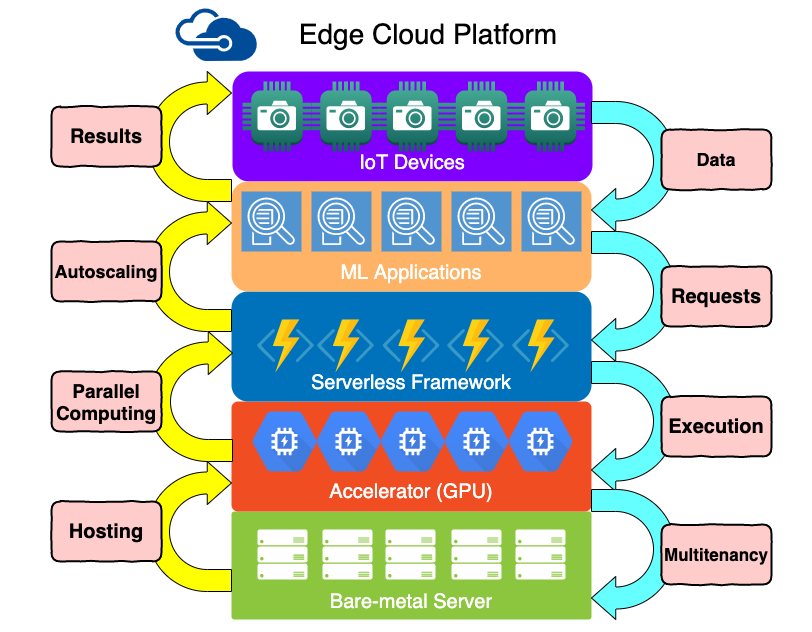
\includegraphics[scale=0.3]{figures/edge_platform}
    \caption{The abstract design of an edge cloud platform leveraging serverless framework and GPUs for executing distributed machine learning applications in IoT settings.
\label{fig:edge}}
\end{figure}

As depicted in Figure~\ref{fig:edge}, we envision an ideal edge cloud platform, to which IoT devices transmit data in batches for training and inference applications. The hierarchy of the platform has five layers: (1) \textbf{bare-metal server} cluster hosts hardware using multitenancy; (2) \textbf{accelerators} (i.e. GPUs) provide computational power by parallel computing; (3) \textbf{serverless framework} autoscales function execution upon the rate of requests; (4) \textbf{machine learning application} receives streaming data from (5) \textbf{IoT devices} and returns results (i.e. classification, regression, etc.)

In this paper, we present STOIC (Serverless TeleOperable Hybrid Cloud) that embraces such designing philosophy. Unique to STOIC, however, is its offloading system which intelligently places the application workload on edge and cloud systems based on its precise prediction of total latency. We consider three major contributions from this work: (1) we design and implement a serverless framework serving IoT requests by leveraging GPU acceleration. (2) we investigate feedback control mechanism and various analytical methodologies to precisely model the unstable edge and public cloud environments. (3) we test the efficacy of using this extended serverless model for machine learning applications that span edge-cloud systems, and empirically evaluate the performance of doing so. Using real workloads and deployments, we find that STOIC reduces the total response time of the benchmark application by 55\% (2.3x speedup), compared with baseline scenario. In the evaluation of duplicator mode, STOIC promptly responds to 95\% (2 GPUs) - 97\% (1 GPU) of requested workloads with the least latency in a 24-hour experiment. 
\fi



\section{STOIC}
\label{sec:stoic}
\begin{figure}
    \centering
    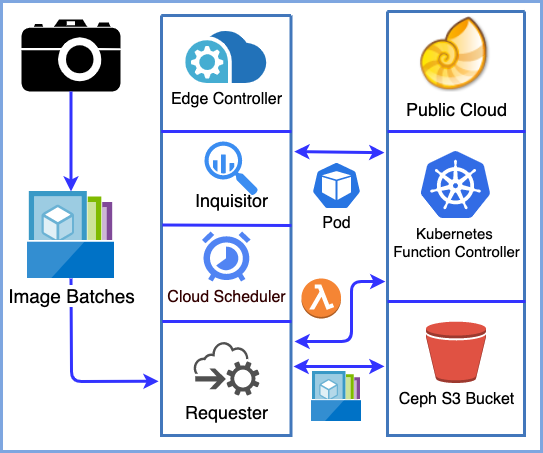
\includegraphics[scale=0.4]{figures/STOIC.png}
    \caption{The STOIC Architecture \label{fig:STOIC}}
\end{figure}

To leverage hardware acceleration and distributed scheduling within a serverless architecture, we have developed STOIC, a framework for executing analytics applications in multi-tier IoT (sensing-edge-cloud) settings. STOIC streamlines the end-to-end process of packaging, transferring, scheduling, executing, and result retrieval for machine learning applications -- using multiple deployment targets (called runtimes). Figure~\ref{fig:STOIC} shows the distributed components of STOIC. Two main pillars comprise a edge controller and a public (or private) cloud.

We have designed the system for image classification applications. In this paper, we investigate its use for processing images from multiple, motion-triggered camera traps (sensors) deployed to monitor wildlife across the Sedgwick Natural Reserve~\cite{ref:sedgwick}.

\subsection{Edge Controller}
The edge controller is a server that runs in an outbuilding at the reserve. It communicates wirelessly with the sensors and triggers analysis/computation upon their arrival. The edge controller is connected to the UCSB campus via a microwave link. When a camera trap detects motion, it takes photos and persists the images in flash storage. Periodically, the sensors transfer saved photos to the edge controller. STOIC runs on the edge controller and its execution is triggered by the arrival of image batches. When a batch arrives, STOIC transfers it to an edge cloud where the tasks are scheduled across +1 cloud components.

As an intermediate computational tier between the sensors and the public cloud, the edge cloud can be placed anywhere, preferably near the edge devices, to lower the response latency for the data processing and analytics applications. It consists of four major components: (1) The \textbf{socket client} continuously listens for requests from the edge controller and receives image batches, (2) the \textbf{cloud scheduler} predicts the total latency based on historical data in a local database for each available runtime, (3) the \textbf{requester} dispatches the workload to the runtime having the least latency and triggers the  serverless function via a RESTful HTTP request either locally at the edge cloud or remotely in the public cloud, (4) the \textbf{inquisitor} deploys all runtimes constantly and records the deployment time respectively in the database. We use the inquisitor to establish the time series for predicting deployment latency.

The edge cloud that we use in this study is deployed 
in our lab on campus, which is connected to both the reserve and the Internet. It consists of a cluster of nine Intel NUCs~\cite{ref:nucs} (6i7KYK), each with two Intel Core i7-6770HQ 4-core processors (6M Cache, 2.60 GHz) and 32GB of DDR4-2133+ RAM connected via two channels. The cluster is managed using the Eucalyptus cloud system~\cite{ref:euca}, which mirrors the Amazon Web Services (AWS) interfaces for Elastic Compute Cloud (EC2) to host Linux virtual machine instances and Simple Storage Service (S3) to provide object storage.
 
 \subsection{Public/Private Cloud}

To investigate the use of the serverless architecture with hardware accelerators, we employ a shared, multiuniversity, GPU cloud, called  Nautilus~\cite{ref:nautilus}, as our remote cloud system. Nautilus is an Internet-connected, HyperCluster research platform developed by researchers at UC San Diego, the National Science Foundation, the Department of Energy, and multiple, participating universities globally.  Nautilus is designed for running data and computationally intensive applications and uses Kubernetes~\cite{ref:k8s} to manage and scale containerized applications. It also uses Rook~\cite{ref:rook} to integrate Ceph~\cite{ref:ceph} for data storage. As of March 2020, Nautilus consists of 176 computing nodes across the US and a total of 524 GPUs in the cluster. All nodes are connected via a multi-campus network. In this study, we consider Nautilus as a public cloud that enables us to leverage hardware acceleration (GPUs) in the serverless architecture to serve edge devices. 

One major challenge we face with such deployments is hardware heterogeneity and performance variability. On Nautilus, we have observed 44 different types of CPU (e.g. Intel Xeon, AMD EPYC, among others) and 9 GPU types (e.g. Nvidia 1080Ti, K40, etc.). Both CPUs and GPUs of different types have different performance characteristics. Besides, ceph storage is run on dedicated nodes that distributed globally.

This heterogeneity impacts application execution time (which STOIC attempts to predict) in three significant ways. First, different CPU clock rates affect the transfer of datasets from the main memory to GPU memory. Second, there is significant latency and variable performance between runtimes and the storage service (which hold the datasets and models). Third, the multi-tenancy of nodes (common in public cloud settings) allows other jobs to share computational resources with our applications of interest at runtime. 

These three factors negatively affect our goal of designing STOIC, which is to efficiently execute IoT applications with minimum latency. With STOIC, we address these challenges to build a novel scheduling system that adapts to this variability. Moreover, to reduce heterogeneity and ensure repeatability of our results, we confine nodes and GPUs in the UCSD region.
%we use node affinity~\cite{ref:nodeAffinity} to confine the nodes only in the UCSD region. This configuration effectively reduces the heterogeneity of the cluster and ensure the reliability of the following experiments.

\subsection{Runtime Scenarios}
To schedule machine learning tasks across hybrid cloud deployments, we define four runtime scenarios: \textbf{(A)} \textit{edge} - A VM instance on the edge cloud with AVX2~\cite{ref:avx} support; \textbf{(B)} \textit{cpu} - A Kubernetes pod on Nautilus containing a single CPU with AVX2~\cite{ref:avx} support; \textbf{(C)} \textit{gpu1} - A Kubernetes pod on Nautilus containing a single GPU; \textbf{(D)} \textit{gpu2} - A Kubernetes pod on Nautilus containing two GPUs. 
STOIC considers each of these deployment options as part of its scheduling decisions. Users can parameterize STOIC with their choice of deployment or allow STOIC to automatically schedule their applications.


\subsection{Execution Time Estimation}
 As depicted in Figure~\ref{fig:STOIC}, 
the STOIC socket client executes in the edge 
cloud and listens for requests from the edge controller (machine learning job requests). After a preset period (parameterizable but currently set to an hour), STOIC estimates total response time~($T_r$) of a requested batch, based on 4 different runtime scenarios. The total response time ($T_s$) includes data transfer time~($T_t$), runtime deployment time~($T_d$) and the corresponding processing time~($T_p$).
 
 \subsubsection{Transfer time~($T_t$)} measures the time spent in transmitting a compressed batch of images from the edge controller to edge cloud and public cloud. We calculate transfer time as ${T_t = F_b / B_c}$ where $F_b$ represents the file size of batch and $B_c$ represents the bandwidth at the moment provided by a bandwidth monitor at the edge controller. 
 
 \subsubsection{Runtime deployment time~($T_d$)} measures the time Nautilus uses to deploy requested kubeless function. Since the scarcity of computation, it is common that multi-GPU runtime takes longer to deploy than single-GPU and CPU runtimes. Note that, for \textit{edge} runtime, the deployment time zeroes out since STOIC executes the task locally in the edge cloud.
 
\begin{figure}
    \centering
    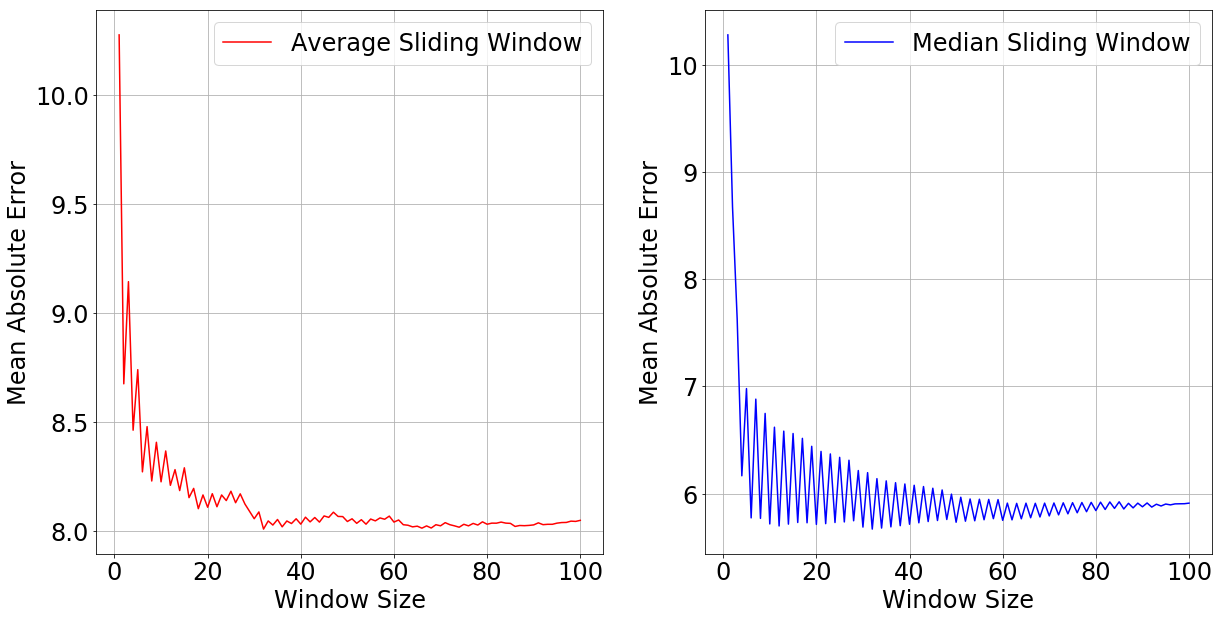
\includegraphics[scale=0.18]{figures/deployment}
    \caption{The Mean Absolute Error (MAE) of deployment time for the \textit{gpu1} runtime. The x-axis is window (history) size. The left subplot is MAE when STOIC uses average sliding window, the right subplot is MAE when STOIC uses median sliding window.
\label{fig:deployment}}
\end{figure}

 
\begin{table}
\centering
\scriptsize
\resizebox{\columnwidth}{!}{
\begin{tabular}{|c|c|c|c|} 
\hline
& & \textbf{Optimal} & \textbf{Minimum}  \\
\textbf{Modeling} & \textbf{Runtime} & \textbf{Window Size} & \textbf{MAE}  \\
\hline
AutoReg & cpu & 15 & 8.977 \\
\hline
AutoReg & gpu1 & 15 & 9.605 \\
\hline
AutoReg & gpu2 & 15 & 17.918 \\
\Xhline{2\arrayrulewidth}
Avg. SW & cpu & 33 & 7.714 \\
\hline
Avg. SW & gpu1 & 31 & 8.006 \\
\hline
Avg. SW & gpu2 & 91 & 16.52 \\
\Xhline{2\arrayrulewidth}
Med. SW & cpu & 13 & \textbf{5.96} \\
\hline
Med. SW & gpu1 & 31 & \textbf{5.668} \\
\hline
Med. SW & gpu2 & 27 & \textbf{14.48} \\
\hline
\end{tabular}
}

\caption{Mean Absolute Error for three time series modeling methods: auto-regression (AutoReg), average sliding window (Avg. SW), and median sliding window (Med. SW). Median sliding window achieves the lowest minimum MAE at optimal window size (that with the lease MAE) for all three runtimes. \label{tab:deployment}}
\end{table}
 

We observe significant variation in deployment time on Nautilus for different times of the day. To accurately predict deployment time, we analyze deployment times as a time series using three methods: (1) auto-regression modeling, (2) average sliding window, and (3) median sliding window. We then compare the minimum 
Mean Absolute Error (MAE) from each to select the best modeling methodology. 

We consider a time series of 1244 data points for each runtime. Figure~\ref{fig:deployment} shows representative analytics for \textit{gpu1} deployment time, in which MAE oscillates as window size varies. We observe that the median sliding window reaches lower minimum MAE than average sliding window at optimal window size. As listed in Table~\ref{tab:deployment}, all three runtimes achieve the lowest minimum MAE using median sliding window. Therefore, STOIC adopts this methodology for deployment time prediction. 

To form a control-loop feedback mechanism, STOIC constantly calibrates the optimal sliding window size while executing, based on the most current deployment time series logged by the inquisitor. The number of data points used in analytics (i.e. 100 by default) and the interval of calibration (i.e. every 10 executions by default) are both parameterizable, in the consideration of tuning between performance and accuracy. 
 
\subsubsection{Processing time~($T_p$)} is the execution time of a specific machine learning task and the target of task scheduling across the hybrid cloud. STOIC formulates a linear regression on execution time histories and uses it to predict processing time, based on the batch size. Specifically, we use Bayesian Ridge Regression~\cite{ref:brr} due to its robustness to ill-posed problems (relative to ordinary least squares regression~\cite{ref:ols}). STOIC queries the database for the most recent processing time data (e.g. 10 data points) for each regression. This ensures that the parameters of the regression line reflect the current runtime performance.
 
As part of our investigations into this approach, we have found that this approach is highly susceptible to outliers. The root cause is sporadic congestion and maintenance (for nodes, networking, etc.) of the public cloud. Deviating significantly from the average, outliers skew the regression line and overestimate the runtime latency for extended periods of time (due to the windowing approach). We thus update the regression using a random sample consensus (RANSAC) technique~\cite{ref:ransac}, which iteratively removes outliers from the regression.
 
 \begin{figure}
    \centering
    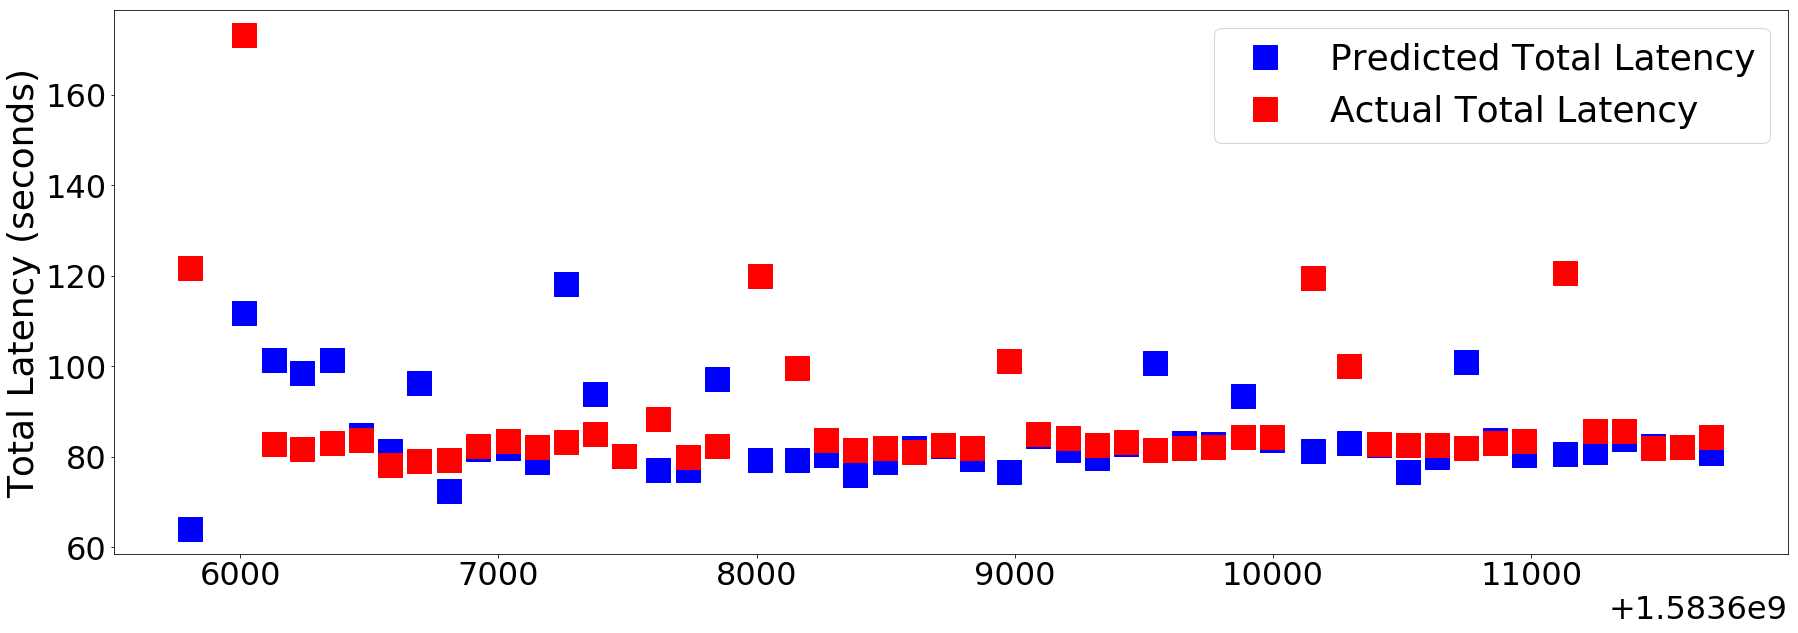
\includegraphics[scale=0.12]{figures/timeline.png}
    \caption{The comparison of predicted and actual total latency on 50 \textit{gpu1} benchmark executions with 150-image batch size. The x-axis is the epoch time and the y-axis is the total latency. \label{fig:timeline}}
\end{figure}

\begin{table}
\centering
\scriptsize
\resizebox{\columnwidth}{!}{
\begin{tabular}{|c|c|c|c|} 
\hline
 & \textbf{Deployment $T_d$} & \textbf{Processing $T_p$} & \textbf{Total $T_s$}  \\
\hline
First Half & 42.7\% & 11.2\% & 15.8\% \\
\hline
Second Half & 29.2\% & 5.3\% & 9.2\% \\
\hline
\end{tabular}
}

\caption{The percentage mean absolute error (PMAE) of deployment, processing and total latency.  \label{tab:timeline}}
\end{table}
 
 \subsubsection{Adaptability}
 
To verify that STOIC's estimation of execution time captures the actual latency of the public cloud, we repeatedly execute our application 50 times with 150-image batch using the \textit{gpu1} runtime. Depicted in Figure~\ref{fig:timeline}, we observe that actual total latency varies significantly and predicted total latency has a non-negligible difference from the actual total latency at the beginning of the experiment. However, over time, as STOIC learns the various latencies of the system, the difference is significantly reduced. In Table~\ref{tab:timeline}, we report the percentage mean absolute error (PMAE), which we compute as the MAE divided by mean latency. The decrease in all three PMAE values in the second half of the execution trace also shows STOIC's adaptability.
 

 \subsection{Implementation}

Considering performance and interface, we implement STOIC using Golang~\cite{ref:golang}. Golang provides high performance execution (vs scripting languages) and a user-friendly interface~\cite{ref:client-go} to Kubernetes and MySQL database. STOIC currently supports machine learning applications developed using the TensorFlow framework~\cite{ref:tensorflow} and can adapt to other machine learning libraries by extending the runtime environment.
 
For our serverless architecture, STOIC integrates kubeless~\cite{ref:kubeless} and Docker~\cite{ref:docker} on the Nautilus Cloud. As a Kubernetes-native serverless framework, kubeless uses the Custom Resource Definition (CRD)~\cite{ref:crd} to dynamically create functions as Kubernetes custom resources and launches runtimes on-demand. For specific machine learning tasks that STOIC executes, we use Docker to build customized runtime images that we upload to Docker Hub~\cite{ref:dockerhub} in advance. When the function controller at Nautilus Cloud receives a task request, it pulls the latest image from Docker Hub before launching the function. This deployment pipeline makes the runtime flexible and extensible for evolving applications. 
 
To create a consistent serverless environment, we install and configure minikube~\cite{ref:minikube} and kubeless~\cite{ref:kubeless} on the edge cloud. They enable the edge cloud to execute and respond to serverless function requests in the same manner as Nautilus. To further reduce the deployment time on the minikube cluster, STOIC creates a standby pod to serve the incoming request upon application invocation. In our experiments, it effectively helps the edge cloud gain the advantage in the function startup time. 

To leverage the computational power of the CPU systems available in the edge and public cloud, we compile Tensorflow with AVX2, SSE4.2~\cite{ref:avx} and FMA~\cite{ref:fma} instruction set support. From our previous test result in~\cite{ref:stoic}, we observe significant speed-up from the customized library on CPU runtime. Therefore, we use this Tensorflow configuration on both the edge cloud and Nautilus.
 
To enable GPU access by serverless functions, we build a container with NVIDIA Container Toolkit~\cite{ref:nvidia}. This includes the NVIDIA runtime library and utilities which link serverless functions to NVIDIA GPUs. We also install CUDA 10.0 and cuDNN 7.0 to support machine learning libraries.
 
 
 \subsection{Workflow}

\begin{figure}[t] \centering 
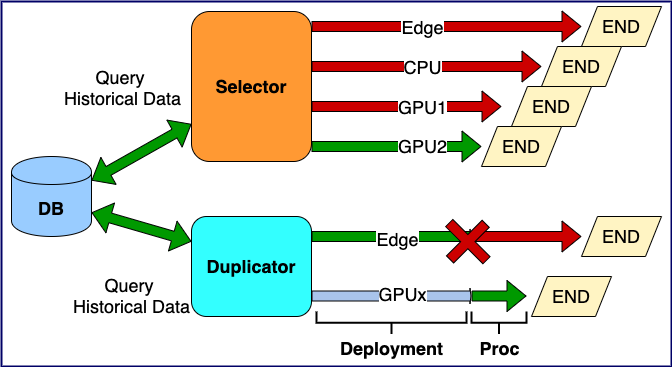
\includegraphics[scale=0.33]{figures/selector_duplicator.png}
\caption{The selector and duplicator modes of STOIC. 
\label{fig:duplicator}}
\end{figure}

The STOIC workflow is as follows: based on the three time components, STOIC predicts the total response times~($T_s$) of the four deployment options. As in the basic \textbf{selector} mode, the scheduler selects the runtime with the shortest estimated response time. Seen in Figure~\ref{fig:duplicator}, the edge cloud then schedules only one request, including the payload of compressed image batch and runtime information. Upon execution, the edge cloud triggers the serverless function locally if the choice is the \textit{edge} runtime. Such deployment is common when a batch of images is small. 

For large batch sizes, STOIC typically schedules one of the three public runtime options. For these three scenarios, the edge cloud first requests the deployment on the public cloud. It then sends the payload to public cloud storage. The public cloud then deploys the runtime on nodes that satisfy the node affinity configuration. To handle unforeseen deployment failure, we implement retry mechanism using exponential back-off delays. Starting at 100 milliseconds, STOIC waits 2X length of time for retrying the deployment on Nautilus. After 10 failed attempts, STOIC claims timeout and returns an error. From our experiments, this mechanism greatly reduces manual intervention and successfully deploys most runtime in a timely manner.
 
Once Nautilus successfully deploys the serverless function, it informs the edge cloud's requester to trigger the function via an HTTP request. To cope with the cold starts~\cite{ref:coldstart}, STOIC triggers the function with the least amount of input data to ensure the function caches the model in memory. When the task completes, the requester retrieves the results and runtime metrics, and transmits them back to the edge controller. Finally, the edge cloud logs the results and metrics to the database for use in later predictions. 

We observe from Table~\ref{tab:timeline} that the unstable deployment time of GPU runtimes significantly affects the accuracy of prediction made by STOIC. To address the issue, we reconfigure STOIC into the \textbf{duplicator} mode demonstrated in Figure~\ref{fig:duplicator}. Based on the historical data, the duplicator runs workload on edge cloud and GPU runtimes concurrently, and halts the edge cloud execution if the remaining time at edge cloud is longer than the expected processing time ($T_p$) at the GPU runtime once it completes deployment. This ``lagging decision'' mechanism reduces the variability of deployment time in the prediction. STOIC only has to consider processing time, which is more accurately predicted, to deploy tasks. Note that duplicator is less energy-efficient because it runs tasks regardless of latency prediction and may waste cloud resources by killing the function in the middle. 

In addition, the inquisitor running in background deploys all runtime scenarios on the public cloud and logs deployment time in the database for prediction. We set a timeout (i.e. 10 minutes) for unresponsive nodes. That is, inquisitor marks the runtime unavailable when the deployment hits the set timeout. Instead of ignoring such runtime, the inquisitor keeps requesting all runtimes across public cloud and resume the runtime's availability if the following deployment is successful.

A final component is the regression initiator which performs bootstrapping. Extended from the initial version, we enable STOIC to take application name and versioning information as input. Once a new application is deployed or the existing application is updated, the regression initiator automatically executes two tasks based on the current application and version for each runtime scenario. These two data points initialize the incoming regressions and predictions across the edge and public cloud.



\section{Evaluation}
\label{sec:results}
In this section, we empirically evaluate STOIC's performance on image
processing tasks. We implement the application as a serverless function for
STOIC to schedule and execute.

In each experiment, we use STOIC's scheduler to determine which resource to
use for function execution (among a small set of feasible choices). We then
run the function on \textit{all} resources and compare the choice made by
STOIC to the best (shortest duration) execution across all possible choices.

\subsection{Experimental Setup}

The image processing application that we use as a benchmark classifies animal
images from a wildlife monitoring system.
%called ``Where's The Bear"
%(WTB)~\cite{ref:wtb}. ``Where's The Bear" is an end-to-end distributed data
%acquisition and analytics system that automatically analyzes camera trap
%images collected by cameras sited at the Sedgwick Natural
%Reserve~\cite{ref:sedgwick} in Santa Barbara County, California. The WTB
The 
deployment includes an ``edge controller'' located near the cameras that are
used to acquire the image data before it is transmitted over a slow network
link to either a private cloud located at a research facility located
approximately 50 miles from the site or to Amazon AWS for web
hosting. In this work, we explore using the Nautilus distributed GPU
cloud~\cite{ref:nautilus} along with the edge cloud to optimize image
classification on a convolutional neural network (CNN)~\cite{ref:cnn}
implemented by Tensorflow and Scikit-learn~\cite{ref:scikit}. 

In total, there are five classes that we consider: Bird, Fox, Rodent, Human
and Empty. Since class size is unbalanced due to the frequency of animal
occurrences, we up-sample minority classes (e.g. fox) using the Keras
ImageDataGenerator~\cite{ref:keras}. Doing so ensures that the classification
model is not biased. We resize every image in the WTB dataset to $1920 \times
1080$, and for each class, the dataset contains 251 images used to train the
CNN model. Once model training is complete, the application stores this model
in hdf5 format in cloud storage at both edge cloud (disk storage) and Nautilus
(a shared volume in a Ceph file system). 

To minimize transfer overhead, we move images from 
the wildlife refuge
%Sedgwick 
to Nautilus in
batches rather than one-at-a-time. To better harness the multiple GPU runtime,
the application spawns a process (worker) for each GPU and adds all images in
a batch to a shared asynchronous queue. Upon the execution, workers remove
images (one at a time) from the shared queue until it is exhausted. This
mechanism ensures multiple GPUs evenly divide the workloads and achieve
quasi-linear acceleration at the application level, where the perfect linear
speed-up is unattainable because of model loading and memory transfer
overhead~\cite{ref:multi_gpu}. 


\iffalse
\subsection{Deployment Options}

We explore four different deployment options on STOIC: 
\begin{itemize}
\item a node of the edge cloud, 
\item on the controlling cpu (an x86 processor) that Nautilus uses to move
data in and out of one or more GPUs,
\item on one GPU in Nautilus,
\item on two GPUs in Nautilus.
\end{itemize} %put in the names here? cjk
On the edge cloud, the application can begin immediately when a camera delivers an image batch.  To use Nautilus, however, the image batch must first traverse the network from the edge cloud to Nautilus (thereby incurring an additional transfer time) and then Nautilus must schedule a ``pod'' (containing either one or two GPU in this study) before the Nautilus CPU or any GPU can begin running.  We define the time that Nautilus requires for pod scheduling as ``deployment time.''~\footnote{Note that Nautilus currently allows non-priviledged users to request up to 8 GPUs, but the deployment times for requests of greater than 2 are usually large as to make them superfluous. That is, a GPU request for more than two GPUs is rarely, if ever successfully, satisfied in the shortest possible time.} Finally, the run time is the time required by a resource (edge cloud cpu, Naultius cpu, on Nautilus GPU, two Nautilus GPUs) to complete the CNN training.  

We do not explore the possibility of overlapping transfer time, deployment time, and run time and we do not model the time required to return the trained model to the edge cloud. Thus the total response time is the sum of the transfer time, the deployment time, and the run time for an image batch. On the edge, the transfer times and deployment times are zero.
\fi



\begin{figure}[t] \centering 
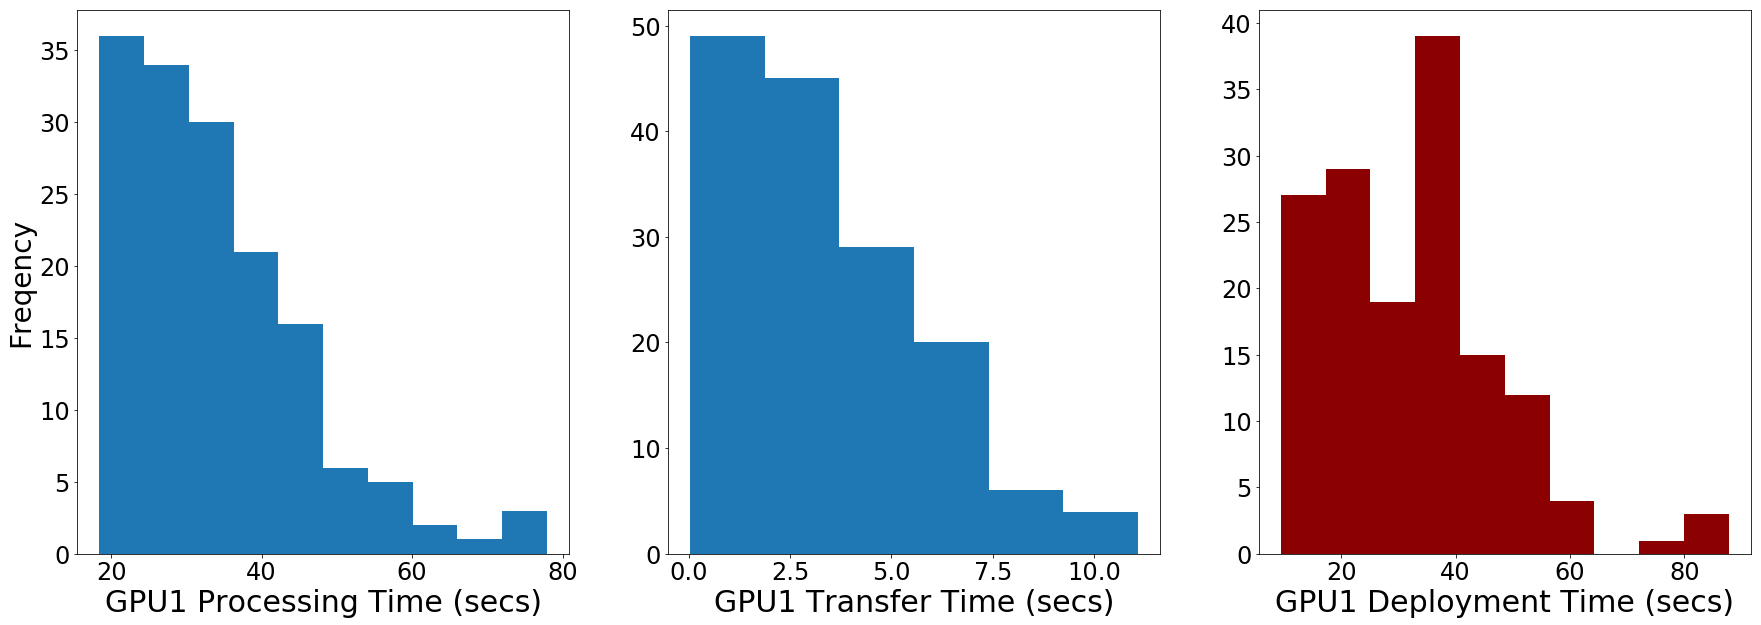
\includegraphics[scale=0.125]{figures/gpu1_latency.png}
\caption{The distribution of three components in total response time~($T_s$) of 150 executions on GPU1 runtime: Processing time ($T_p$), Deployment time ($T_d$) and Transfer time ($T_t$). The x-axis represents the time range, while the y-axis is the frequency of executions. The deployment time, which is depicted in the red histogram, is volatile and error-prone to prediction.
\label{fig:breakdown}}
\end{figure}

In the experiment, we model the batch size using simulator that leverages
historical data derived from the WTB image corpus from 2013 to 2017 and the
arrival rate of images at the cameras. Figure~\ref{fig:breakdown} shows an
example histograms for processing time, transfer time and deployment time on
Nautilus for GPU1 runtime using 150 batches drawn from the simulator. On the
x-axis, we show the elapsed time for processing time, transfer time, and
deployment time respectively.  Note that processing time and transfer time are
relatively stable compared to deployment time. 

\subsection{Selector Evaluation}

We evaluate the STOIC Selector over a 24-hour time period consisting of 162
image batches, the sizes of which are drawn randomly from the simulator. Each
batch is executed on the edge cloud, on the Nautilus CPU, on one Nautilus GPU
and on two Nautilus GPUs. Over the test period, the STOIC Selector chooses the
fastest (lowest total response time) from among these four options $149$ times
out of the $162$ runs or $92\%$ of the time. That is, STOIC correctly
identifies the fastest option with a success rate of $92\%$.

Further, the optimal selection (i.e. an oracle selection that is $100\%$
correct) would have resulted in an aggregate total latency of $10022$ seconds
and the worst case aggregate latency as $35940$ seconds compared to a STOIC
aggregate latency of $10770$ seconds.  Thus STOIC achieves an aggregate
latency that is $5.3\%$ slower than optimal, but $70\%$ ($3.33$) times faster
than the worst case. Table~\ref{tab:selector} summarizes these results. In the
table, we report the success rate, the percentage of optimal, and the
percentage of worst case aggregate response times achieved by STOIC. 

\begin{table}[t] 
\begin{centering}
\captionsetup{justification=centering}
\scriptsize
\resizebox{\columnwidth}{!}{
\begin{tabular}{|c|c|c|} 
\hline
\textbf{Success Rate} & \textbf{versus Optimal} & \textbf{versus Worst Case}\\
\hline
$92\%$ & $105\%$ & $30\%$ \\
\hline
\end{tabular}
}

\end{centering}
\caption{
STOIC Selector results. The success rate is the percentage of correct decisions
(out of 162 trials) made by STOIC.  ``Optimal'' shows the percentage of the
optimal selection aggregate response time and ``Worst Case'' shows the percentage of the worst case 
selection aggregate response time made by STOIC.}
\label{tab:selector}
\end{table}

We further analyze the data points where STOIC made erroneous selections and
found two sources of error. First, the most error occurs around two batch
sizes where the total response times of runtime have approximately same
latency. To be specific, the edge and GPU runtimes cross over at 35 image
batch size, and 90 image batch size for the GPU1 and GPU2 runtimes. At these
cross-points, the close predictions of latency lead to incorrect selection.
Second, the deployment times for GPU runtime are volatile and error-prone to
prediction. As a representative instance, Figure~\ref{fig:breakdown}
demonstrates the distribution of processing time ($T_p$), transfer time
($T_t$) and deployment time ($T_d$) of GPU1 runtime. We observe geometric
distribution from the histogram of processing time and transfer time, whereas
deployment time varies irregularly with many outliers. These two phenomenons
lead to mistaken selections in the experiment.

\subsection{Duplicator Evaluation}

Note that the edge cloud node is not a shared resource -- it is dedicated to
the application. It is implemented using inexpensive hardware that is
connected to standard 120 VAC power (in a closet in a management building
located at the refuge).
%at Sedgwick).  
As a result,
it is possible to use the edge cloud for \textit{every} batch even when it is
not the fastest.  

Put another way, there is no cost to running the edge cloud speculatively
while data is transferring to Nautilus and the application waits for Nautilus
to deploy pods for the cpu and GPUx runtimes. If STOIC (using Selector)
predicts that Nautilus will be faster, and STOIC is correct, the work on the
edge cloud is ``duplicate work'' which is unnecessary. However because of the
deployment variability, it may be that the edge cloud speculative execution
finishes ahead of that runtime scheduled to Nautilus.

However, unlike the edge cloud node, Nautilus is a shared resource.  Thus we
do not wish to ``waste'' execution time on Nautilus unnecessarily. Thus, in
this setting, the cost of duplicate work on the edge is minimal compared to
the cost of potentially duplicate work on Nautilus. If this were not true, we
would simply launch the job both at the edge and on Nautilus and use whichever
finished first.

Thus we explore a second scheduling strategy that attempts to minimize total
response time in light of the following assumptions.
\begin{itemize}
\item Duplicating unneeded work on the edge carries no penalty.
\item Duplicating unneeded work in Nautilus is expensive.
\item The STOIC predictions (initial and after transfer and deployment) will be used to
choose the resource that yields the fastest response time while using the
Nautilus resources parsimoniously.
\end{itemize}
We call the STOIC scheduler that attempts to minimize response times under these assumptions -- the Duplicator.

Further, we noticed that the Naultilus cpu was seldom a good choice in
practice. The application must ``pay'' for the transfer and incur the
deployment time variability to acquire a CPU that is almost equivalent to the
edge node CPU.  Thus, in the ``real world'' version of the STOIC scheduler for
WTB, we use the Duplicator with Nautilus GPUs only.

The scheduling algorithm starts the task on the edge cloud node and also
begins the transfer to Nautilus. It then waits for the Nautilus deployment
time and, when the pod is fully deployed, it predicts whether to use the
freshly acquired GPU or GPUs (i.e. to ``switch'' to the GPU(s)) or to abandon
the request and to complete the job on the edge.  To do so, STOIC must predict
the \textit{remaining} edge time at the moment the GPU pod is deployed, and
compare this remaining time to the predicted GPU processing time.  

The Duplicator prediction is \textit{conditional} upon the amount of time that
has elapsed during transfer and deployment to Nautilus. If STOIC predicts that
the GPU pod will start and complete their processing before the edge completes
what remains of the job, it allows the Nautilus and edge cloud executions to
execute concurrently. If the Nautilus job completes first, the edge cloud
execution is terminated.  Otherwise, if the edge cloud execution finishes
first (i.e. the prediction was incorrect) then the Nautilus job is terminated
(and the time between the start of the Nautilus job and the end of the cloud
job is ``wasted'' Nautilus time).

Alternatively, when STOIC predicts that the edge cloud will finish first, it
returns the GPU resources to Nautilus and run only the edge cloud job. If the
Nautilus job would have completed first (i.e. the conditional prediction in
favor of the edge is incorrect) then the time between when the Nautilus job
would have finished and the time that the edge cloud job completes is
additional delay (compared to having made a correct prediction).

Thus, choosing incorrectly (i.e. a failure) occurs when the actual completion
time exceeds the time of the runtime corresponding to the minimum prediction
(in either edge or GPU case) made by STOIC. That is, a ``failure'' for the
Duplicator occurs when STOIC makes a conditional choice (i.e. continue on edge
or to include Nautilus) and the choice results in a longer \textit{actual}
response time than the one not chosen. Table~\ref{tab:comparison} shows the
performance of the Duplicator using the edge and one GPU and, separately, the
edge and two GPUs from Nautilus. We duplicate the results for the Selector
from Table~\ref{tab:selector} for comparison purposes.

\begin{table}[t] 
\centering
\captionsetup{justification=centering}
\scriptsize
\resizebox{\columnwidth}{!}{
\begin{tabular}{|c|c|c|c|} 
\hline
& \textbf{Success Rate} & \textbf{versus Optimal}  & \textbf{versus Worst Case}\\
\hline
Selector  & $85\%$ & $108\%$ & $45\%$\\
\hline
Duplicator Edge vs GPU1 & $97\%$ & $102\%$ & $45\%$\\
\hline
Duplicator Edge vs GPU2 & \textbf{$95\%$} & \textbf{$101\%$} & \textbf{$45\%$} \\
\hline
\end{tabular}
}

\caption{
The comparison of Selector and Duplicators}
\label{tab:comparison}
\end{table}

These results are both expected and surprising. As expected, restricting the
choice to edge and a single Nautilus request and using a conditional
prediction at deployment time (as opposed to a ranking at the beginning) as a
success criterion improves the success rate dramatically. We do not claim that
Duplicator is better than Selector in terms of success rate. Instead,
Duplicator enables a more dependable scheduling strategy for the
classification application based on
conditional predictions rather than resource ranking. Surprisingly, however,
requesting 2 GPUs improves both success rate and aggregate response time
relative to choosing one.

This result surprised us for two reasons. First, because there was greater
deployment variance and a larger mean deployment time for two GPUs, we expect
that the edge (which is more predictable) would generate a greater success
rate, but a larger aggregate response time. Put another way, we expected that
STOIC would make safer predictions favoring the edge in the two GPU case, but
the cost of this safety would be greater aggregate response time. Empirically,
however, we observe that STOIC ``risks'' predicting the two GPU deployment
more frequently, but that it amortizes this risk effectively because the two
GPU execution is faster.

Note that the cost is not large. In practice, the 
application
%WTB project 
will use the one
GPU case to get a better success rate at the cost of $1\%$ in aggregate
response time.  However, it is interesting that STOIC is able to make this
risk-reward trade-off explicit. Note also that the worst case is unchanged.
This result indicates that there are unusually bad response time, but that
\textit{all} STOIC scheduling methods can mitigate them to approximately the
same degree.

We conclude our analysis with a quantification of the savings and unnecessary
loss of Nautilus time that STOIC Duplicator is able to achieve.
Table~\ref{tab:savings} shows the savings and loss of Nautilus time that are
realized by the Duplicator heuristic.

%
%error Duplicator makes
%with respect to the STOIC conditional predictions.
%We define Mean Deadline Error (MDE) as the mean over prediction (in seconds)
%made by STOIC in the case the actual total response time exceeds the predicted
%total response time.
%$MDE = \frac{1}{n}\sum(L_g - L_e)
%\,|\ if \ L_g > L_e \ \& \ R_s = GPUx $, where $L_g$ is the latency of GPU
%runtime, $L_e$ is the latency of edge cloud, $R_s$ is the actual runtime by
%STOIC. 
%We define the ``Mean Overprediction Error'' (MOE) as the average
%overprediction that Duplicator makes when it fails to choose the fastest
%option.
%Based on the experiment data, the MOE for edge and one Nautilus GPU is $27$ seconds 
%and for edge and two Nautilus GPUs it is $44$ seconds.
%Thus, when Duplicator fails to choose correctly, the average ``miss''
%is under a minute.
%

\begin{table}[t] 
\centering
\scriptsize
\resizebox{\columnwidth}{!}{
\begin{tabular}{|c|c|} 
\hline
\textbf{STOIC Choice} & \textbf{Nautilus Savings (+) or Loss (-)}\\
\hline
edge & $+1393$s\\
\hline
1 gpu & $-440$s\\
\hline
2 gpus & $-257$s\\
\hline
\end{tabular}
}

\caption{
Nautilus savings (positive values) and loss (negative values) for STOIC Duplicator. Savings are the time returned to Nautilus due to edge execution. Loss is the time used on Nautilus unnecessarily due to a faster edge execution. All units are seconds. In the 2 GPU case, the time is for both GPUs.}
\label{tab:savings}
\end{table}

Recall that the total optimal time (the time associated with the minimum
execution of each batch) is $10022$ seconds. The positive values in the table
indicate the total time returned to Nautilus (that would have otherwise been
used) by selecting the edge for execution.  Note that these savings correspond
to the results shown in Table~\ref{tab:comparison} for the Duplicator. That
is, they are the savings that STOIC was able to achieve while implementing a
schedule within either $1\%$ or $2\%$ of optimal.  The loss (negative values)
shows the amount of Nautilus time that was used unnecessarily. That is, when
STOIC Duplicator chose conditionally to use the GPU or GPUs and the edge
finishes first, the elapsed time on Nautilus is unnecessarily ``lost.''
Clearly from the table, Duplicator saves more Nautilus time than it loses.
Thus, we infer that STOIC in duplicator mode optimizes the time to solution
(Table~\ref{tab:comparison}) while utilizing the expensive Nautilus resource
efficiently (Table~\ref{tab:savings}) by using the edge cloud node
speculatively.  


% (47.43\% to the
%mean gpu2 runtime latency). This result implies that the unstable deployment
%time of GPU runtimes significantly affects the accuracy of prediction made by
%STOIC. 

%To address the above issue, we reconfigure STOIC into the duplicator mode
%demonstrated in Figure~\ref{fig:duplicator}. Based on the historical data,
%the selector makes prediction and only execute workload at the runtime with
%least total latency, whereas the duplicator runs workload on edge cloud and
%GPU runtimes concurrently, and halts the edge cloud execution if the
%remaining time at edge cloud is longer than the expected processing time
%($T_p$) at the GPU runtime once it completes deployment.
%Table~\ref{tab:success} shows the conditions of success rate for duplicators:
%only when STOIC switches to GPU runtime and GPU runtime has higher latency,
%we label the execution as a failure. Notice that case 2 and 6 are success
%cases, because edge cloud has higher priority in the system (e.g. proximity,
%stability, etc.) and it completes the execution ahead of GPU runtime. Under
%the duplicator mode, STOIC is able to make right selection between edge cloud
%and GPU1 runtime and promptly respond to the requests 96.7\% of times and the
%total latency further drops to 7877.72 seconds . 
%
%\begin{figure}[t] \centering 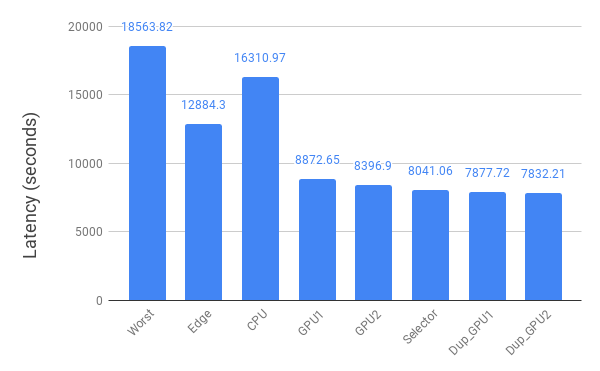
\includegraphics[scale=0.42]{latency.png}
%\caption{The Total Latency of the worst scenario, single runtimes, selector
%and duplicators. } \label{fig:latency} \end{figure}
%
%We next analyze the duplicator of edge cloud versus gpu2. According to the MDE
%metric, gpu2 runtime has more variable deployment and processing time compared
%to gpu1 runtime, which possibly leads to a lower success rate of selection.
%The analytics of the data proves this assumption that STOIC only makes right
%selection between edge cloud and gpu2 runtime by 94.8\% of times, 1.9\% lower
%than being with gpu1 runtime. However, as depicted in the
%Figure~\ref{fig:latency}, the total latency of single gpu2 runtime is shorter
%than the total latency for single gpu1 runtime. We argue that even though
%STOIC make slightly more mistakes in this mode, the duplicator of gpu2 forms a
%faster and more efficient dispatching system. Demonstrated in the
%Table~\ref{tab:comparison}, duplicator of gpu2 runtime achieves the lowest
%average latency (50.86 seconds) and highest speedup (2.37x). We plan to
%investigate runtimes with more GPUs and the trade-off between the
%predictability and efficiency of system as future work.

\iffalse
Table~\ref{tab:success} summarizes the possible success failure cases for the
Duplicator.
\begin{table}[t] 
\centering
\captionsetup{justification=centering}
\scriptsize
\resizebox{\columnwidth}{!}{
\begin{tabular}{|c|c|c|c|} 
\hline
\textbf{\makecell{Predicted GPU \\Lower Latency}} & \textbf{Switch to GPU} & \textbf{\makecell{Actual GPU \\Lower Latency} } & \textbf{Case Label}\\
\hline
Yes & Yes & Yes & Success \\
\hline
Yes & Yes & No & Success \\
\hline
Yes & No & Yes & \textbf{Failure} \\
\hline
Yes & No & No & Success \\
\hline
No & Yes & Yes & Success\\
\hline
No & Yes & No & Success \\
\hline
No & No & Yes & \textbf{Failure} \\
\hline
No & No & No & Success \\
\hline
\end{tabular}
}
\caption{
Duplicator success/failure cases for STOIC.}
\label{tab:success}
\end{table}

\begin{algorithm}[]
\caption{Duplicator Success Rate Heuristic}
\label{algo:optimizer}
\SetAlgoLined
\KwData{Executions on Edge and GPUx runtime}
\KwResult{Runtime Selection Labels}
\For{Executions on Edge and GPUx}{
 \eIf{Predicted GPUx $T_s$ $<$ Predicted Edge $T_s$}{
    \eIf{Predicted Edge $T_s$ - (Actual GPUs $T_t$ + Actual GPUs $T_d$)) $\ge$ Predicted GPUx $T_s$}{
    \eIf{Actual GPUx $T_s$ $<$ Actual Edge $T_s$}{SUCCESS}{SUCCESS}
 }{
    \eIf{Actual GPUx $T_s$ $<$ Actual Edge $T_s$}{FAILURE}{SUCCESS}}}
 {
 \eIf{Predicted Edge $T_s$ - (Actual GPUs $T_t$ + Actual GPUs $T_d$)) $\ge$ Predicted GPUx $T_s$}{
    \eIf{Actual GPUx $T_s$ $<$ Actual Edge $T_s$}{SUCCESS}{SUCCESS}
 }{
    \eIf{Acutal GPUx $T_s$ $<$ Actual Edge $T_s$}{FAILURE}{SUCCESS}}
 }
}
\end{algorithm}
\fi


\section{Related Work}
\label{sec:related}
We explored an early design and scheduler for STOIC in~\cite{ref:stoic}.  This
paper extends this workshop paper with a new scheduling system and
consideration of both individual and concurrent edge-cloud placements. In
other related works, we consider recent advances in machine learning
infrastructure leveraging serverless computing, GPU accelerators, and
Kubernetes orchestration service. \cite{ref:serverlessstep} and
\cite{ref:berkeleyserverless} conduct a comprehensive survey on serverless
computing including challenges and research opportunities. We share the same
viewpoint that the use of the serverless execution model will grow for online
training and inference applications. \cite{ref:deepserving} provides a
prototype for deep learning model serving in a serverless platform.
\cite{ref:accelerated} provides another use case for accelerating serverless
functions by GPU virtualization in data centers. Unique in our work, STOIC
extends an existing serverless framework to support GPU acceleration and
distributed function placement across the edge and public clouds.
\cite{ref:evaluation} evaluates several serverless frameworks based on
Kubernetes. We also employ Kubernetes for container orchestration, which is
lightweight, flexible, and developer-friendly.  We concur that Kubernetes is a
promising deployment infrastructure for serverless computing.  

The second relevant domain of related work is image recognition on IoT devices
and edge clouds. \cite{ref:face} compares the processing time of face
recognition between the edge device and IoT, namely smartphones. It concludes
that edge devices perform comparably faster and scales better as the number of
images increases. We agree with this conclusion, and as such, design STOIC to
offload image processing workloads to both edge clouds and public clouds.
\cite{ref:DDNN} proposes a distributed deep neural network that allows fast
and localized inference at the edge device using truncated layers of a neural
network. \cite{ref:cooperative} defines edge cloud offloading as a Markov
decision process (MDP) whose objective is to minimize the average processing
time per job. Based on this setting, it provides a novel approximate solution
to MDP with a one-step policy iteration. These works are complementary to
STOIC and we are considering how to incorporate them into the system as part
of future work.

Also complimentary to STOIC, are tracing, testing, repair, and profiling tools
(which STOIC can leverage) for serverless systems. Multiple works track causal
dependencies across distributed serverless deployments for use in
optimization, placement, and data
repair~\cite{ref:repairdata,deptracing19,gammaray17,aws-xray}.
FaaSProfiler~\cite{ref:profile} provides a tool for testing and profiling
STOIC as a FaaS platform. \cite{ref:security} proposes a security solution
that applies reinforcement learning (RL) to provide secure offloading to the
edge nodes to prevent jamming attacks. These related systems can be combined
with STOIC to provide a robust serverless ecosystem for distributed IoT
devices.



\section{Conclusion}
\label{sec:conc}
In this paper, we propose a framework, called STOIC, for executing machine
learning applications in IoT-cloud settings using the serverless
architecture. STO\-IC integrates an edge controller, an edge cloud, and a public
cloud with GPU acceleration. When the scheduler at the edge controller
receives a batch of images from open field camera traps, it predicts the total
response time for processing the batch based on batch size and historical log
data. In the selector mode, STOIC schedules the task to the runtime with the
least predicted latency. In the duplicator mode, STOIC co-schedules the task
on the edge cloud and GPU runtime in the public cloud. If the latter is
deployed and predicted to be faster, the edge cloud job is terminated.
Otherwise, STOIC terminates the public cloud job and 
completes the task on the edge cloud.
This mode further optimizes the selection process by avoiding volatile
deployment times.

We present the design principles, implementation details, the feedback control
mechanism, and different modeling methodologies to address the variability in
edge and public cloud deployments. Our empirical evaluation demonstrates STOIC
can schedule tasks on local and remote deployments to achieve a speedup of
3.3x versus our baseline scenario. STOIC's success rate for prediction
placement  ranges from 92\% to 97\% for the application and datasets that we
study. 

As part of future work, we plan to investigate substituting RANSAC with
Gradient Boosting Regression Trees (GBRT) to capture the non-linearity in the
processing time due to heterogeneous hardware across deployment options
(runtimes). We also plan to investigate model check-pointing in duplicator
mode to better utilize computational resource on edge cloud and to improve the
overall performance of the STOIC system.


% cannot include this until paper is unblinded
%\section*{Acknowledgments}
%This work has been supported in part by NSF (CNS-1703560, CCF-1539586,
%ACI-1541215), ONR NEEC (N00174-16-C-0020),
%and the AWS Cloud Credits for Research program.
%This work was performed in part at the University of California Natural Reserve System Sedgwick Reserve DOI: 10.21973/N3C08R.



% \bibliographystyle{ACM-Reference-Format}
\bibliographystyle{IEEEtran}
\bibliography{ref_acm}

\end{document}


